\documentclass[11pt,a4paper]{article}
\usepackage[a4paper,top=0.85in,bottom=1in,left=1.1in,right=1.1in]{geometry}
\usepackage{amsmath,amssymb,amsthm}
\usepackage{mathtools}
\usepackage{graphicx}
\usepackage{float}
\usepackage{booktabs}
\usepackage{hyperref}
\usepackage{cleveref}
\usepackage[round]{natbib}
\usepackage{microtype}

\newcommand{\R}{\mathbb{R}}
\newcommand{\E}{\mathbb{E}}
\newcommand{\KL}{\mathrm{KL}}
\newcommand{\OT}{\mathrm{OT}}
\DeclareMathOperator*{\argmin}{arg\,min}
\DeclareMathOperator*{\argmax}{arg\,max}
\newcommand{\transpose}{^{\!\top}}
\newcommand{\defeq}{\coloneqq}
\newtheorem*{remark}{Remark}

\title{Sinkhorn-HTI: an entropic substitute for HTI's inner-loop $c$-transform}
\author{David Nelischer\\[2pt] \small Optimal Transport, Institut Polytechnique de Paris\\ \small Spring 2026}
\date{}

\IfFileExists{numbers.tex}{\newcommand{\nOuter}{2001}
\newcommand{\theSeed}{5}
\newcommand{\maxiterLBFGS}{10}
\newcommand{\nllLbfgs}{6.98}
\newcommand{\nllEnt}{12.05}
\newcommand{\cdLbfgs}{0.0158}
\newcommand{\cdEnt}{0.0130}
\newcommand{\wallLbfgs}{12461}
\newcommand{\wallEnt}{3808}
\newcommand{\wallRatio}{3.3}
}{%
  \newcommand{\nOuter}{2001}%
  \newcommand{\theSeed}{5}%
  \newcommand{\maxiterLBFGS}{10}%
  \newcommand{\nllLbfgs}{\textsc{pending}}%
  \newcommand{\nllEnt}{\textsc{pending}}%
  \newcommand{\cdLbfgs}{\textsc{pending}}%
  \newcommand{\cdEnt}{\textsc{pending}}%
  \newcommand{\wallLbfgs}{\textsc{pending}}%
  \newcommand{\wallEnt}{\textsc{pending}}%
  \newcommand{\wallRatio}{\textsc{pending}}%
}

\begin{document}
\maketitle

\begin{abstract}
Hyperparameter Trajectory Inference \citep[HTI;][]{amad2026hti} fits a
conditional Lagrangian-OT surrogate by alternating between a potential /
transport / spline update and an outer metric update. The potential
update requires a per-batch Kantorovich $c$-transform whose hard form
is a non-convex minimization over $y_1$, which \citet{amad2026hti}
solve with an inner L-BFGS loop. The first-order condition of the
entropic dual is closed form: the soft $c$-transform, which replaces
the inner loop by a single LogSumExp over the mini-batch; the
transport-map regression target becomes the entropic barycentric
projection of \citet{pooladian2021entropic}. On the semicircles
benchmark of \citet{amad2026hti} at paper budget, the entropic variant
($\varepsilon=3\times 10^{-3}$) reaches held-out
$\mathrm{NLL}=\nllEnt$ and circle distance $\mathrm{CD}=\cdEnt$ (mean
deviation from the unit circle) against $\nllLbfgs$ and $\cdLbfgs$
for L-BFGS, and trains
$\wallRatio\times$ faster. At fixed $\varepsilon>0$ the entropic OT
value carries an $\mathcal{O}(\varepsilon)$ bias \citep{pal2024difference}.
\end{abstract}

\section{Introduction}
\label{sec:intro}

HTI \citep{amad2026hti} learns how a neural network's conditional output
distribution $p_{\theta_\lambda}(y\mid x)$ evolves with a continuous
hyperparameter $\lambda$, given a sparse set of observed marginals. The
method (Neural CLOT) extends the neural Lagrangian optimal-transport
framework of \citet{pooladian2024nlot} to the conditional setting,
and is trained by the alternating procedure of Algorithm~1 in
\citet{amad2026hti}. Inside this alternation, the Kantorovich potential $g$
is updated against a semi-dual objective whose $c$-transform requires,
for each source sample $y_0$ in a mini-batch, solving an inner
minimization over candidate target points $y_1\in\R^d$. \citet{amad2026hti} solve this via a short L-BFGS run
warm-started from the transport-map network $T$ (10 iterations for
semicircles, cf \citealt{amad2026hti}).

\smallskip
Entropic OT yields a closed-form soft $c$-transform that replaces
this inner minimization, at the cost of a bias controlled by a
regularization strength $\varepsilon$. On the semicircles benchmark we implement both
variants on top of the same network code and compare them at paper
budget (seed~\theSeed{}, $N_{\text{outer}}=\nOuter$).

\section{Background}
\label{sec:background}

For probability measures $\mu,\nu\in\mathcal{P}(\R^d)$ with finite
second moments and a continuous nonnegative cost $c$, the Kantorovich
semi-dual \citep{villani2008ot}
\begin{equation}
\OT_c(\mu,\nu)=\sup_{g\in L^1(\nu)}\int g^c\,\mathrm{d}\mu
+\int g\,\mathrm{d}\nu,
\qquad
g^c(y_0)\defeq\inf_{y_1\in\R^d}\bigl\{c(y_0,y_1)-g(y_1)\bigr\}
\label{eq:hard-ct}
\end{equation}
holds with one inner minimization per source $y_0$ in a single
potential $g$. Adding a $\KL$ penalty against $\mu\otimes\nu$ to the primal,
\begin{equation}
\OT_c^\varepsilon(\mu,\nu)\defeq
\inf_{\pi\in\Pi(\mu,\nu)} \int c\,\mathrm{d}\pi
+\varepsilon\,\KL(\pi\,\|\,\mu\otimes\nu),
\label{eq:eot-primal}
\end{equation}
yields a strongly concave dual whose first-order condition in $f$ at
fixed $g$ has a closed form
\citep{peyre2019book},
the \emph{soft $c$-transform}
\begin{equation}
g^{c,\varepsilon}(y_0)
\defeq -\varepsilon\log\int
\exp\!\bigl(\tfrac{g(y_1)-c(y_0,y_1)}{\varepsilon}\bigr)\,
\mathrm{d}\nu(y_1),
\label{eq:soft-ct}
\end{equation}
with $g^{c,\varepsilon}\to g^c$ as $\varepsilon\to 0$ and an
$\mathcal{O}(\varepsilon)$ bias on the OT value \citep{pal2024difference}. HTI applies \cref{eq:hard-ct} to conditional measures
$\mu_k(\cdot\mid x)$ and $\mu_{k+1}(\cdot\mid x)$ at consecutive
anchor times $t_0 < \cdots < t_T$, with cost $c(y_0, y_1 \mid x)$
defined as the least action of a learned conditional Lagrangian
$\mathcal{L}(q, \dot q \mid x) = \tfrac12 \dot q\transpose G(q \mid x)
\dot q - U(q \mid x)$ along paths $q$ joining $y_0$ to $y_1$.

\smallskip
For each source $y_0$ in a mini-batch, the resulting inner
minimization over $y_1$ is solved by a short L-BFGS run warm-started
from a transport-map network $T$ (Algorithm~1, line~10 of
\citealt{amad2026hti}). We keep the
density-bias potential $U$, the learned metric $G$, and the spline
head $S$ (a small MLP that proposes the candidate path $q$ used in
the action integral) exactly as in \citet{amad2026hti}.

\section{The substitution}
\label{sec:substitution}

\paragraph{Derivation.}
Starting from the entropic dual of \cref{eq:eot-primal},
\begin{equation*}
\OT_c^\varepsilon(\mu,\nu)=\sup_{f,g}\Bigl\{\int f\,\mathrm{d}\mu
+\int g\,\mathrm{d}\nu
-\varepsilon\iint \exp\!\bigl(\tfrac{f(y_0)+g(y_1)-c(y_0,y_1)}{\varepsilon}\bigr)\,
\mathrm{d}\mu(y_0)\,\mathrm{d}\nu(y_1)+\varepsilon\Bigr\},
\end{equation*}
the objective is strictly concave in $f$ at fixed $g$ for $\varepsilon>0$
\citep{peyre2019book}, and the first-order condition in $f$
gives $f^{*}=g^{c,\varepsilon}$. Replacing $\nu$ in \cref{eq:soft-ct}
by its mini-batch empirical version yields the empirical soft
$c$-transform
\begin{equation}
\hat g^{c,\varepsilon}_{B}(y_k^{(i)}\mid x)
= -\varepsilon\,\log\sum_{j=1}^{B} \exp\!\Bigl[\,
\tfrac{g_{\theta_g,k}(y_{k+1}^{(j)}\mid x)
-c(y_k^{(i)},y_{k+1}^{(j)}\mid x)}{\varepsilon}\,\Bigr].
\label{eq:sinkhorn-hti}
\end{equation}
The standard $1/B$-normalized form differs by a constant
$\varepsilon\log B$ that is $y_k$- and $\theta_g$-independent and so
vanishes in the dual-loss gradient.

\paragraph{Map-regression target.}
Replacing line~10 of Algorithm~1 in \citet{amad2026hti} by
\cref{eq:sinkhorn-hti} also changes the regression target for the
transport-map network. HTI's baseline regresses $T_{\theta_T,k}$
against the inner L-BFGS argmin; the natural entropic counterpart is
the barycentric projection \citep{pooladian2021entropic}, i.e., the
conditional expectation of the target under the same soft entropic
plan, with the same $\exp((g-c)/\varepsilon)$ weights as
\cref{eq:sinkhorn-hti}:
\begin{equation}
\hat T^\varepsilon(y_k^{(i)}\mid x)
= \sum_{j=1}^{B}w_{ij}\,y_{k+1}^{(j)},\qquad
w_{ij}\propto\exp\!\Bigl(\tfrac{g_{\theta_g,k}(y_{k+1}^{(j)}\mid x)
-c(y_k^{(i)},y_{k+1}^{(j)}\mid x)}{\varepsilon}\Bigr).
\label{eq:bary}
\end{equation}
\Cref{eq:bary} is the barycentric projection of the entropic OT plan
\citep{pooladian2021entropic} and recovers the hard argmin as
$\varepsilon\to 0$. In HTI's baseline, $T_{\theta_T,k}$
plays two coupled roles per outer step: warm-starting the inner
L-BFGS run, and being regressed against its argmin. The entropic
variant breaks this coupling: the barycentric projection in
\cref{eq:bary} is computed from the cost matrix alone, independently
of $T$. All other HTI components (metric, potential, spline head, outer
update) are unchanged.

\begin{remark}
\Cref{eq:sinkhorn-hti} replaces the per-sample L-BFGS argmin by a
batch-wise LogSumExp (the $-\varepsilon\log\sum_j\exp(\cdot)$ in
\cref{eq:sinkhorn-hti}). L-BFGS is tighter for well-converged $g$
with a good $T$ warm start.
\end{remark}

\section{Experiments}
\label{sec:experiments}

\paragraph{Framework and budget.}
We reimplement HTI in JAX/Equinox. Outer budget
$N_{\text{outer}}=\nOuter$, inner budget $N_{\text{inner}}=10$, and
$\maxiterLBFGS$ L-BFGS iterations per source all match the choices made in \citet{amad2026hti}. Both methods use mini-batch $B=64$, which puts their per-step
compute in the same range: the entropic step builds a single
$B \times B$ cost matrix, while the L-BFGS variant runs $B$ short
inner optimizations of $\maxiterLBFGS$ iterations each. The data has four conditions, three anchor times
$t\in\{0,0.5,1\}$, and $100$ samples per condition.

\paragraph{Architectures and hyperparameters.}
Architectures match Table~8 of \citet{amad2026hti} with two
deliberate changes: a smaller spline MLP ($[512,512]$ vs $[1024,1024]$)
and
an explicit eigenvalue floor $\lambda_{\min}=0.3$ (the paper states
none); other Lagrangian hyperparameters $(\alpha, h_y)=(0.05, 0.05)$
follow the original choices ($\alpha$ is the density-potential
strength, $h_y$ is the KDE bandwidth used inside it). The entropic regularization is fixed at
$\varepsilon=3\times 10^{-3}$.

\paragraph{Outer metric optimizer.}
The values used in \citet{amad2026hti} and the released code
\citep{amad2026hticode} ($\eta_G=5\times 10^{-3}$, and gradient clip
$1$) produced a late-training metric-loss blow-up in our runs
(see \Cref{sec:discussion}); we therefore use a constant
$\eta_G=5\times 10^{-4}$ and tighten gradient-norm clipping to $0.25$.
The official HTI code \citep{amad2026hticode} was only released after running the experiments and building the code; relative to its semicircles configuration we
make two further changes: mini-batch $B = 64$ (release: $1024$) and
eigenvalue floor $\lambda_{\min} = 0.3$ (release: $0.1$). The
smaller $B$ is forced by our limited compute budget and the
entropic step's $\mathcal{O}(B^2)$ memory cost.

\paragraph{Evaluation.}
Held-out metrics are computed at $t\in\{0.25,0.75\}$: (i) NLL via a
Gaussian-KDE of surrogate samples (bandwidth $0.05$) evaluated at new ground-truth samples per condition, and (ii) the
circle distance
\[
\mathrm{CD} \defeq \E\bigl[\,\bigl|\,\|y - \text{center}\|_2 - 1\,\bigr|\,\bigr],
\]
the mean deviation of generated points from the unit circle of the
corresponding semicircle condition.
Seed~\theSeed{} was selected as the best-performing of five
exploratory seeds at $N_{\text{outer}}=400$.

\paragraph{Training dynamics.}
\Cref{fig:training} shows the four losses logged each outer iteration
(potential, map, spline, and outer metric). Both methods drive their
losses down over roughly the first 500 iterations and then plateau. The
L-BFGS dual and metric panels carry occasional spikes: the inner
problem is non-convex, so a metric step can shift which local minimum
L-BFGS lands on, and the per-sample dual estimate jumps. The entropic
dual is a LogSumExp and stays smooth. The two map losses are not
directly comparable: our regression target depends on which target
samples fall in the current mini-batch, whereas the L-BFGS argmin is
batch-independent.

\paragraph{Held-out metrics.}
\Cref{tab:results} reports wall-clock training time, the mean held-out
NLL and CD over the two evaluation times, and the per-time breakdown.
The headline NLL gap is concentrated at $t=0.25$
(closer to anchor $t=0$); the gap at $t=0.75$ is narrower in NLL but reverses on CD.

\begin{table}[H]
\centering
\small
\setlength{\tabcolsep}{4pt}
\IfFileExists{table_results.tex}{\begin{tabular}{l c cc cc cc}
\toprule
& Time (s) & \multicolumn{2}{c}{Mean} & \multicolumn{2}{c}{$t=0.25$} & \multicolumn{2}{c}{$t=0.75$} \\
\cmidrule(lr){3-4} \cmidrule(lr){5-6} \cmidrule(lr){7-8}
Method & $\downarrow$ & NLL $\downarrow$ & CD $\downarrow$ & NLL $\downarrow$ & CD $\downarrow$ & NLL $\downarrow$ & CD $\downarrow$ \\
\midrule
L-BFGS inner solver & 12461 & 6.98 & 0.0158 & 10.13 & 0.0119 & 3.83 & 0.0198 \\
Sinkhorn-HTI, $\varepsilon=3\times 10^{-3}$ & 3808 & 12.05 & 0.0130 & 19.72 & 0.0051 & 4.39 & 0.0210 \\
\bottomrule
\end{tabular}
}{%
\begin{tabular}{l c cc cc cc}
\toprule
& Time (s) & \multicolumn{2}{c}{Mean} & \multicolumn{2}{c}{$t=0.25$} & \multicolumn{2}{c}{$t=0.75$} \\
\cmidrule(lr){3-4} \cmidrule(lr){5-6} \cmidrule(lr){7-8}
Method & $\downarrow$ & NLL $\downarrow$ & CD $\downarrow$ & NLL $\downarrow$ & CD $\downarrow$ & NLL $\downarrow$ & CD $\downarrow$ \\
\midrule
L-BFGS inner solver & \wallLbfgs & \nllLbfgs & \cdLbfgs & \textsc{pending} & \textsc{pending} & \textsc{pending} & \textsc{pending} \\
Sinkhorn-HTI, $\varepsilon=3\times 10^{-3}$ & \wallEnt & \nllEnt & \cdEnt & \textsc{pending} & \textsc{pending} & \textsc{pending} & \textsc{pending} \\
\bottomrule
\end{tabular}%
}
\caption{Semicircles held-out metrics. Mean is the
average over $t\in\{0.25,0.75\}$; wall-clock ratio
$\wallLbfgs/\wallEnt\approx\wallRatio\times$.}
\label{tab:results}
\end{table}

\begin{figure}[!t]
\centering
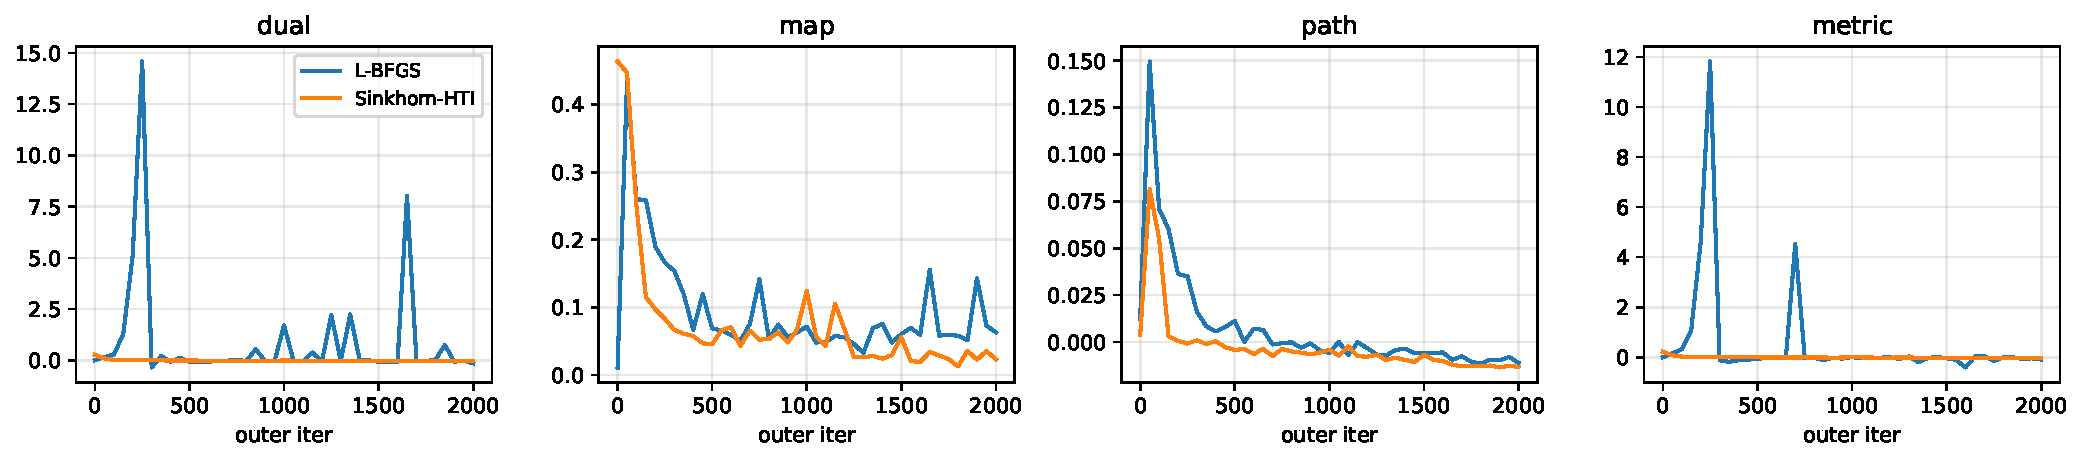
\includegraphics[width=\linewidth]{figs/training_curves.pdf}
\caption{Training-loss trajectories. Panels: dual
$\mathcal{L}_{\text{dual}}$, map $\mathcal{L}_{\text{map}}$, path
$\mathcal{L}_{\text{path}}$, outer-metric $\mathcal{L}_{\text{metric}}$.
Each outer iteration runs one $N_{\text{inner}}$-pass per anchor
interval, giving $2\,N_{\text{inner}}$ inner steps in total. Each
plotted point is the mean over those step losses.}
\label{fig:training}
\end{figure}

\paragraph{Qualitative reconstruction.}
\Cref{fig:trajectories} plots surrogate-predicted trajectories for $12$
starting samples per condition alongside the ground-truth process. Both
methods recover the circular geometry.

\begin{figure}[!t]
\centering
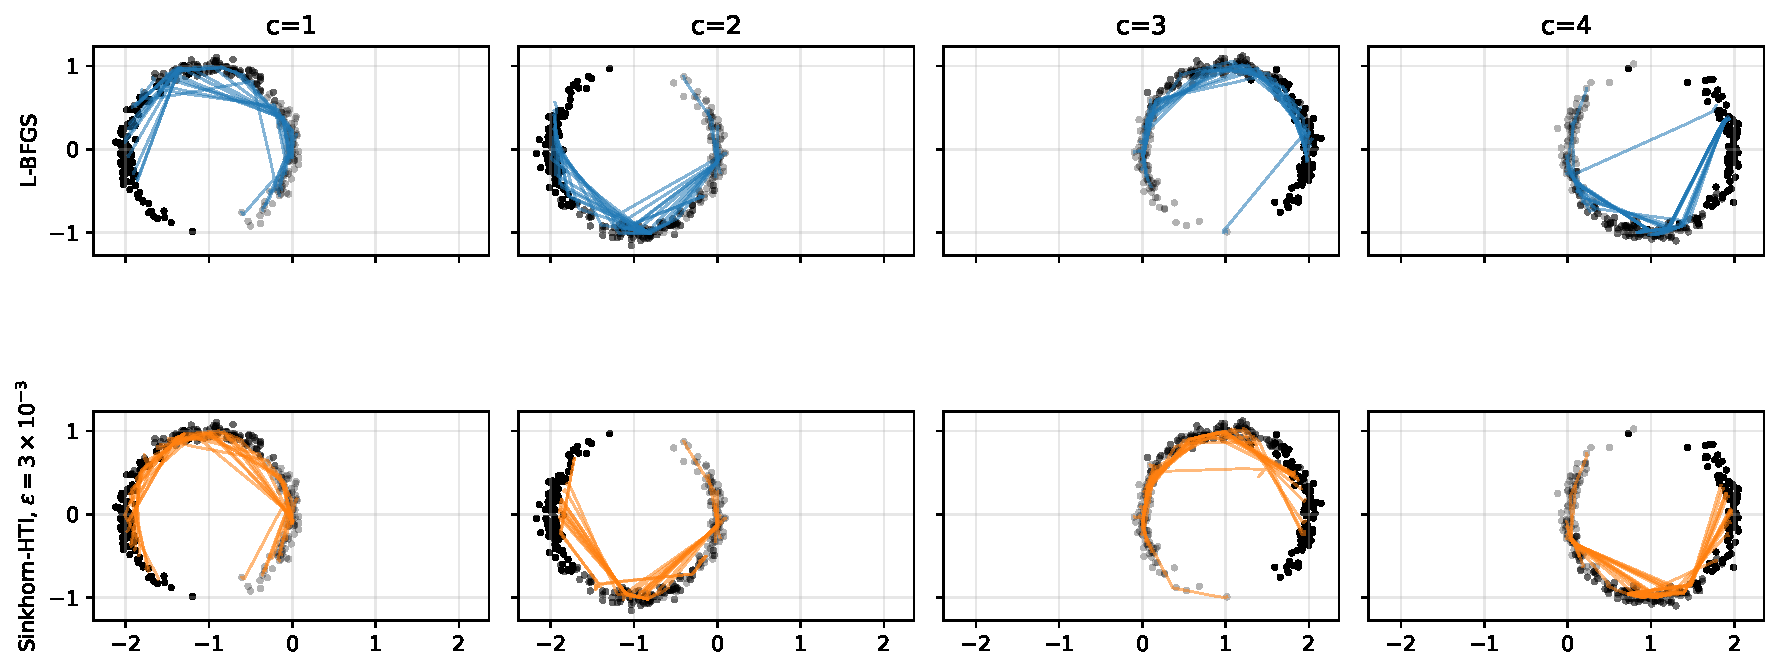
\includegraphics[width=\linewidth]{figs/trajectories_compare.pdf}
\caption{Surrogate trajectories. Dots: ground-truth samples at
$t\in\{0,0.25,0.5,0.75,1\}$ with increasing opacity. Lines:
surrogate paths from composing $T_{\theta_T,k}$ and the spline
head.}
\label{fig:trajectories}
\end{figure}

\section{Discussion}
\label{sec:discussion}

\paragraph{Headline.}
The two methods share architecture, initialization, data, anchor RNG,
batch size, and outer-optimizer schedule, so the gap in
\Cref{tab:results} is attributable to the inner-solver substitution.
L-BFGS attains lower KDE-NLL; the entropic variant attains lower CD
and trains roughly $\wallRatio\times$ faster.

\paragraph{Outer learning rate.}
The metric learning rate and gradient clip used in
\citet{amad2026hti} and the released code \citep{amad2026hticode},
$\eta_G = 5\times 10^{-3}$ and clip $1$, made training unstable in
our runs: the metric loss kept growing late on, and the final spline
drifted off the unit circles. We instead use a smaller
$\eta_G = 5\times 10^{-4}$ and a tighter clip of $0.25$, which keeps
training stable. The entropic variant runs with the same outer-loop
settings, so the comparison only reflects the change in inner
solver.

\paragraph{Inner-solver budget.}
We follow the choice in \citet{amad2026hti} with $\maxiterLBFGS$ L-BFGS iterations. Larger
inner budgets produce a degenerate transport map with $T_{\theta_T,k}$ collapsing to the identity because the converged $y_1^\star$ from L-BFGS sits near its warm start $T(y_0)$,
leaving the map MSE near zero throughout training. The entropic
variant's regression target is the barycentric projection, computed
independently of $T$, and is unaffected.

\paragraph{Lagrangian-strength ablation.}
An exploratory run at $(\alpha, h_y) = (1.0, 0.1)$ substantially
degraded held-out KDE-NLL on both methods: the strong-$\alpha$ regime
over-pulls geodesics toward density ridges, hurting likelihood at
held-out times without however fully breaking CD. The paper's
$(\alpha, h_y) = (0.05, 0.05)$ is the right choice for our optimizer.

\paragraph{Computational cost.}
At matched $B=64$, the entropic inner step is a single
$\mathcal{O}(B^2)$ LogSumExp over the pre-built cost matrix, while
the L-BFGS inner step is $B$ independent per-sample runs of
$\maxiterLBFGS$ iterations each. The L-BFGS variant therefore does
roughly an order of magnitude more cost-function and gradient
evaluations per mini-batch; the measured wall-clock ratio is
$\wallRatio\times$ (\Cref{tab:results}).

\paragraph{Regularization bias.}
At fixed $\varepsilon>0$ the entropic OT value carries an
$\mathcal{O}(\varepsilon)$ bias under standard regularity
\citep{pal2024difference}. The bias on the gradient that drives the
outer metric update is harder to characterize, so we
just pick $\varepsilon=3\times 10^{-3}$ and check the choice
empirically. A sweep of the soft-dual on the Sinkhorn-HTI
components (\Cref{fig:eps-sweep}) confirms that the dual is
essentially flat for $\varepsilon\le 10^{-2}$ and drops sharply for
$\varepsilon\ge 10^{-1}$, so the training $\varepsilon$ is well
within the flat regime.

\paragraph{Independence.}
The entire framework was reimplemented from scratch using only the
\citet{amad2026hti} paper (with help from an LLM); the official
release \citep{amad2026hticode} appeared after the experiments were
done and was consulted only for a few values the paper does not list
(gradient clip, default $B$, eigenvalue floor $\lambda_{\min}$).
The soft $c$-transform substitution itself has no counterpart in
the released code.

\paragraph{Scope.}
HTI's separate limitations (multi-hyperparameter extension, chaotic
dynamics, metric-bias correction) are not adressed by the inner-loop
choice.

\begin{figure}[H]
\centering
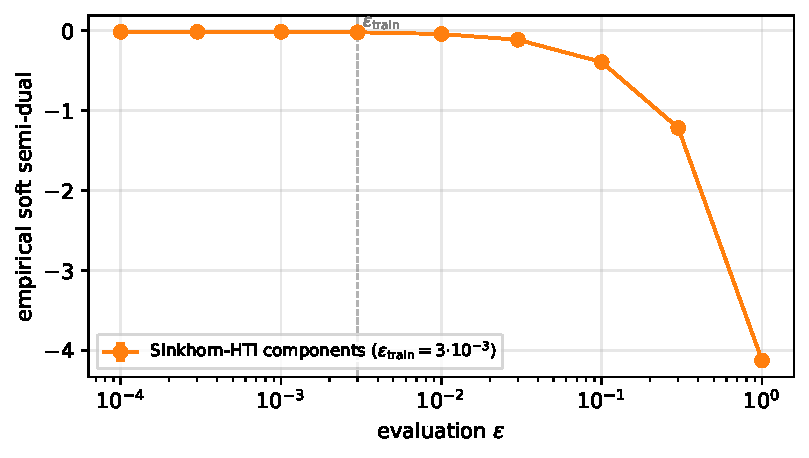
\includegraphics[width=0.55\linewidth]{figs/eps_sweep.pdf}
\caption{Empirical soft semi-dual on the Sinkhorn-HTI
components at varying evaluation $\varepsilon$. Mean over $8$
mini-batches. Vertical line: training $\varepsilon=3\times 10^{-3}$.}
\label{fig:eps-sweep}
\end{figure}

\bibliographystyle{plainnat}
\bibliography{refs}

\end{document}
